\section{Selection Operators}
\label{sec:selection}
This chapter gives an overview of different types of selection operators which are used to select chromosomes from the population for producing offspring. We consider the following selection operators, naming them according to the terminology used by \citeauthor{razali2011genetic} \cite{razali2011genetic}:

\begin{itemize}
	\item Random selection
	\item Proportional roulette wheel selection (Section 4.1)
	\item Rank-based roulette wheel selection (Section 4.2)
	\item Tournament selection (Section 4.3)
\end{itemize}

Random selection picks randomly two parents from the current population, where all chromosomes typically have the same probability of being selected (see \cite{knust2020script}). This means that the fitness value of a chromosome has no influence on its probability of producing offspring. Therefore, random selection is quite straightforward but may not produce optimal results.\par 

In contrast to that, the next three selection operators do consider the fitness values when selecting chromosomes. They will be explained in detail in the sections below.

\subsection{Proportional Roulette Wheel Selection}
\label{subsec:proportional}

In this type of selection, each chromosome has a probability of being selected which is directly proportional to its fitness value. This selection operator is called "roulette wheel" as the probabilities correspond to portions in a roulette wheel. In this way, chromosomes with a larger fitness value are more probable to be selected.\par 

Let $POP$ be the current population and $f_{i}$ be the fitness value of the chromosome $i \in POP$. The selection probability $p_{i}$ for this chromosome $i$ is defined as $p_{i} := f_{i}/ \sum_{j\in POP} f_{j}$, and the accumulated value is calculated as $q_{i} = \sum_{j = 1}^{i} p_{j}$ (see \cite{knust2020script}). To select a chromosome for reproduction, a random number $rand \in [0, 1]$ is drawn: If $rand \leq q_{1}$, the chromosome with the index 1  is selected. Otherwise, one chooses the chromosome with the index $i \geq 2$, where $q_{i - 1} < rand \leq  q_{i}$.\par 

For instance, let us assume that a population contains 4 chromosomes with the fitness values 8, 4, 20, and 32, respectively. The sum of all fitness values is 64. Therefore,  $p_{1} = 8/64 = 0.125$, $p_{2} = 4/64 = 0.0625$, $p_{3} = 20/64 = 0.3125$, and $p_{4} = 32/64 = 0.5$ (see Table \ref{5_1_wheel_selection_data} and Figure \ref{5_1_wheel_selection}). Now the accumulated values have to be calculated: $q_{1} =  0.125$, $q_{2} = 0.125 + 0625 = 0.1875$, $q_{3} = 0.1875 + 0.3125 = 0.5$, and $q_{4} = 0.5 + 0.5 = 1$. If we draw $rand = 0.01$, the first chromosome is chosen, as $0.01 < 0.0625$. If, on the other hand, we draw $rand = 0.8$, then the chromosome with the index $4$ is chosen, as $q_{3} < 0.8 <  q_{4}$. \\

\begin{table}[htp] \centering
	\centering
	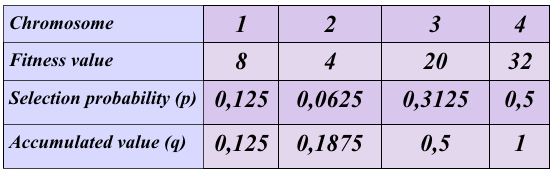
\includegraphics[width=0.5\textwidth]{4_1_wheel_selection_data}
	\caption{Selection probabilities and accumulated values for four chromosomes with fitness values 8, 4, 20, and 32, respectively, for the proportional roulette wheel selection (based on an example by \citeauthor{knust2020script} in \cite{knust2020script}).}
	\label{5_1_wheel_selection_data}
\end{table}


\begin{figure}[htp] \centering
	\centering
	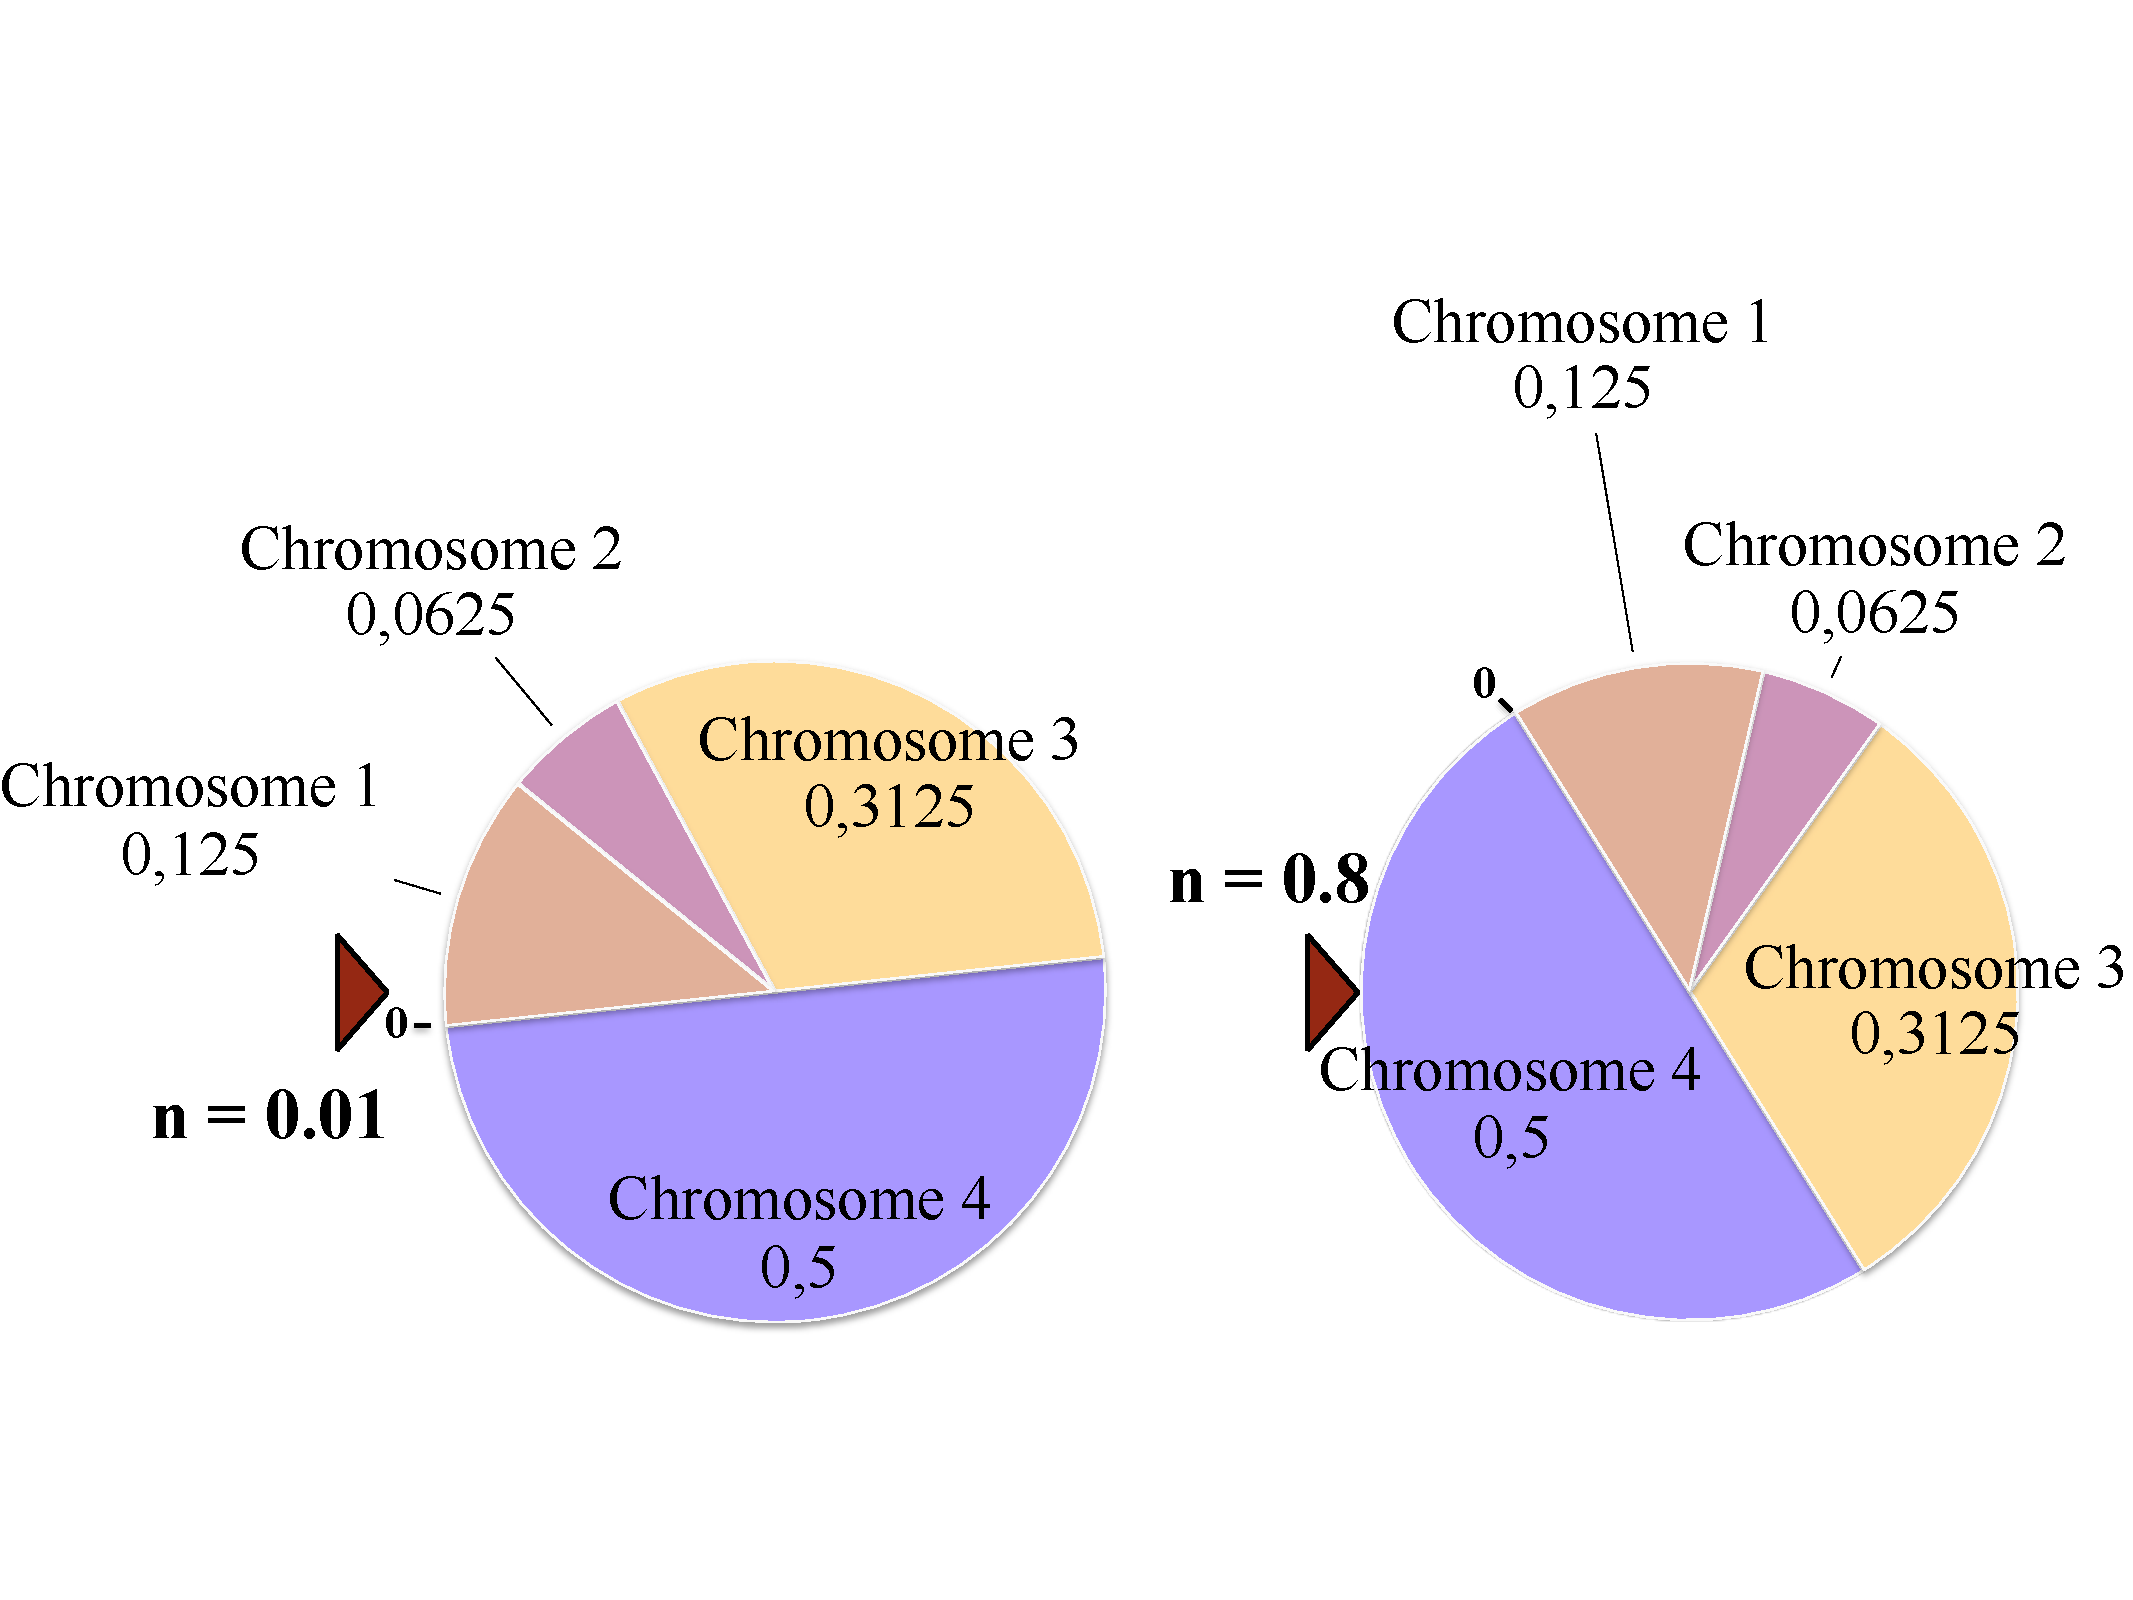
\includegraphics[width=0.6\textwidth]{5_1_roulette_wheel_selection}
	\caption{Selection probabilities in form of a "roulette wheel" for the four chromosomes from Table \ref{5_1_wheel_selection_data}.}
	\label{5_1_wheel_selection}
\end{figure}


Thus, the proportional roulette wheel selection gives a chance to all chromosomes in the population, assigning higher priority to the ones with larger fitness values. On the one hand, the fittest chromosomes are more likely to be selected. This corresponds to the idea of natural selection where the fittest individuals tend to survive. On the other hand, the other chromosomes can still be selected as well. However, \citeauthor{razali2011genetic} \cite{razali2011genetic} pointed out that this selection type has a disadvantage: If an initial population contains a pair of very good (but still not optimal) chromosomes, and if the remainder of the population has relatively low fitness values, then these "good" chromosomes can quickly dominate the whole population. This may cause the genetic algorithm to get stuck in local minima. \par 

Due to this shortcoming, other selection procedures have been developed, where the selection probability is not directly proportional to the fitness value of the chromosomes. They will be described in the following sections.\par

\subsection{Rank-Based Roulette Wheel Selection}
\label{subsec:rank_based}

In the proportional roulette wheel selection, the selection probabilities are defined by the absolute fitness values of chromosomes. In contrast to that, the rank-based roulette wheel selection does not use fitness values for computing the selection probabilities directly. This selection type constructs a ranking of chromosomes instead: Each chromosome $i \in POP$ gets a rank value $r_{i}$, where the chromosome with the lowest fitness value gets the rank $r = 1$, and the chromosome with the largest fitness value obtains the rank $r = |POP|$. The selection probabilities $p_{i}$ for each chromosome $i \in POP $ are calculated according to the defined ranks, namely $p_{i} = r_{i}/\sum_{j \in POP} r_{j}$ (see \cite{knust2020script}). Please note that selection probabilities here can be also considered as portions in a roulette wheel; therefore, this selection type also contains "roulette wheel" in its name.\par  

Let us again consider the example from Section 4.1, i.e. four chromosomes with fitness values $8$, $4$, $20$, and $32$, respectively. The computed ranks for these four chromosomes are: $r_{1} = 2$, $r_{2} = 1$, $r_{3} = 3$, and $r_{4} = 4$. This ranking results in the following selection probabilities: $p_{1} = 2/(2 + 1+ 3 + 4) = 0.2$, $p_{2} = 0.1$, $p_{3} = 0.3$, and $p_{2} = 0.4$ (see Table \ref{5_2_rank_selection_data}). In Figure \ref{5_2_rank_selection}, we compare the selection probabilities for proportional and rank-based roulette wheel selection for this example. Obviously, the chromosomes with lower fitness values have a higher chance of being selected in the rank-based variant than in the proportional one. This can be easily seen by comparing the two charts in Figure \ref{5_2_rank_selection}. For instance, the randomly drawn number $rand = 0.19$ results in selecting chromosome 3 in the proportional roulette wheel selection, whereas the rank-based variant still chooses the first chromosome.\par

\begin{table}[htp] \centering
	\centering
	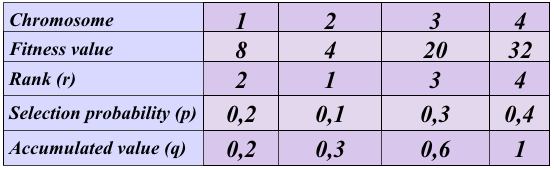
\includegraphics[width=0.5\textwidth]{4_2_rank_selection_data}
	\caption{The selection probabilities and accumulated values for four chromosomes with the fitness values 8, 4, 20, and 32, respectively, for the rank-based selection.}
	\label{5_2_rank_selection_data}
\end{table}

\begin{figure}[htp] \centering
	\centering
	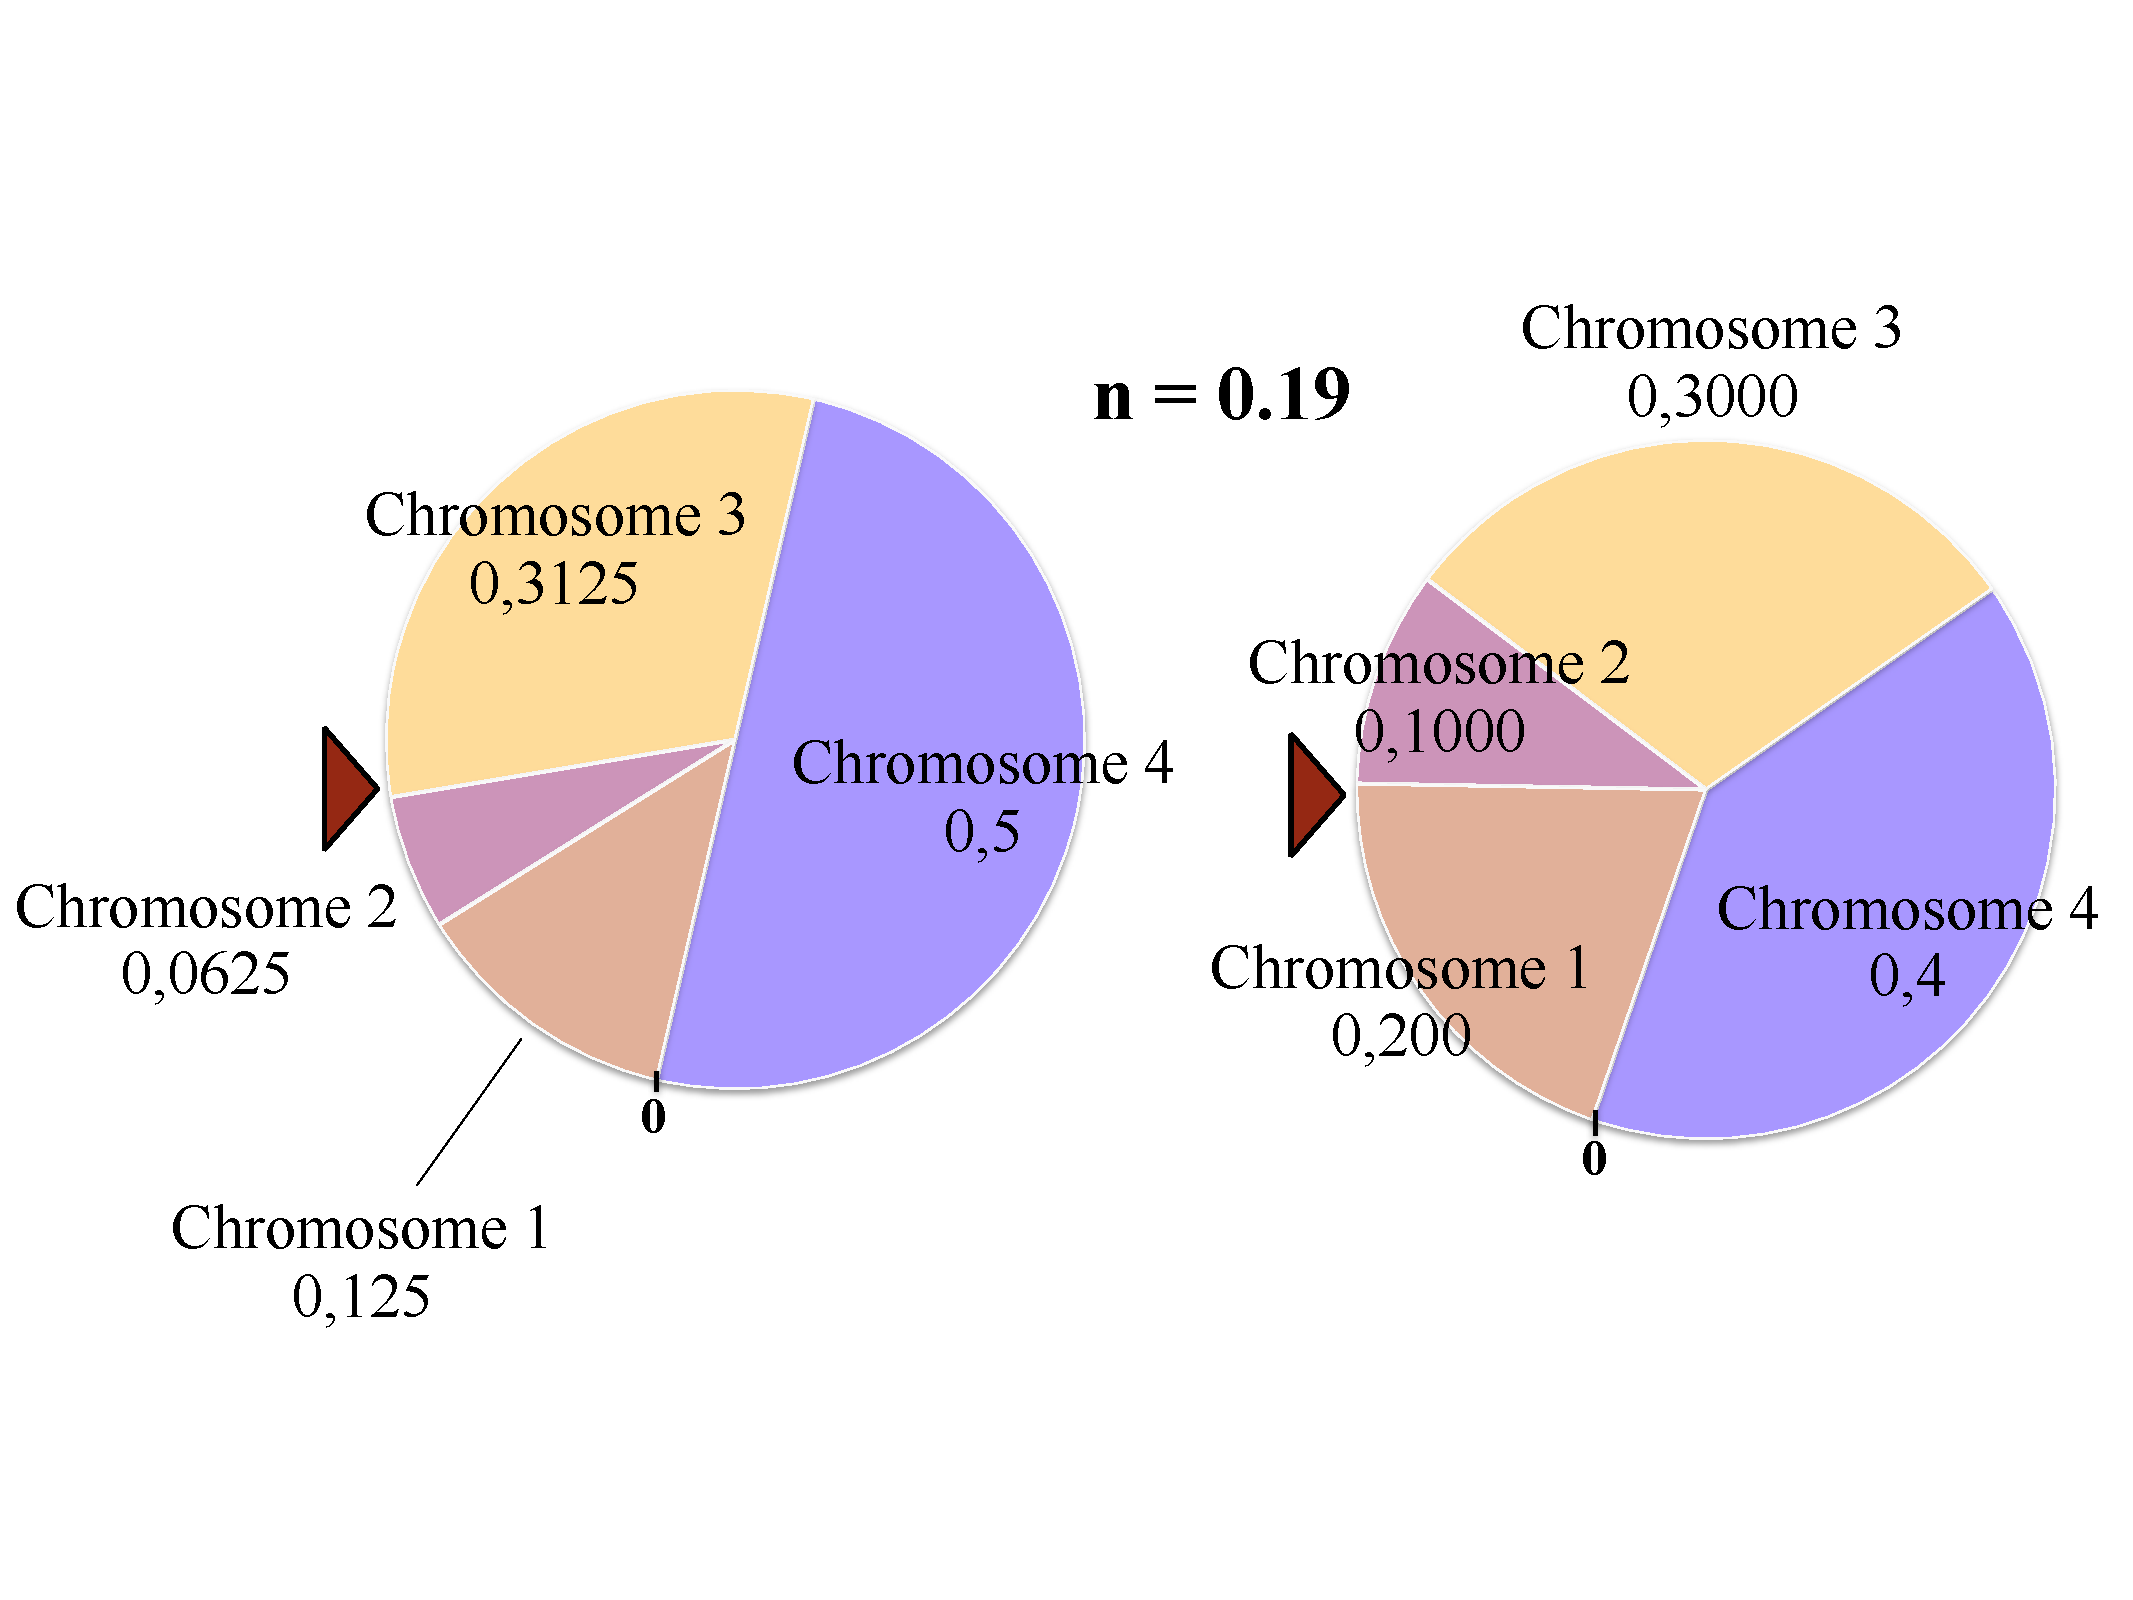
\includegraphics[width=0.6\textwidth]{5_2_rank_selection}
	\caption{Selection probabilities for the proportional roulette wheel selection (left) and the rank-based roulette wheel selection (right) computed for four chromosomes with fitness values 8, 4, 20, and 32, respectively.}
	\label{5_2_rank_selection}
\end{figure}

Therefore, this selection type solves the problem of getting stuck in local minima which can occur in the proportional roulette wheel selection because the influence of the chromosomes with very good fitness values is not so strong anymore. According to \citeauthor{razali2011genetic} \cite{razali2011genetic}, the main disadvantage of this approach is that the population has to be sorted for constructing the ranking which can result in high computational costs. Moreover, there can appear a problem of slow convergence because the selection probabilities of the best chromosomes do not differ so much from the ones of the other chromosomes.\par  


\subsection{Tournament Selection}
\label{subsec:tournament}
The tournament selection considers $p$ randomly chosen chromosomes from the population for selection. Among this group of chromosomes, the one with the highest fitness value is selected. The number of chromosomes $p$ which take part in the tournament can depend on the size of the population. \par 
One possible choice is to set $p$ to a fixed constant. This is for example done in a so-called binary tournament which works with two participants (see \cite{goldberg1991comparative}). Another option is to choose $p$ randomly as well. When choosing $p$, one should consider two effects: On the one hand, if the number of participants is too large, chromosomes with smaller fitness values are selected very rarely because the best chromosomes always take part in the tournament. On the other hand, if $p$ is too small in comparison to the population size, only very few chromosomes take part in the tournament. Especially if the number of generations is not large, this means that a large proportion of the population is never considered for selection. \par
In comparison to the previous two selection types, the tournament selection gives a greater chance for the chromosomes with low fitness values (if $p$ is not large). The chromosomes are taken into the tournament independent from their fitness values. Therefore, the first advantage of the tournament selection is that it cannot be easily trapped in local minima. Secondly, the implementation is easier: It does not require additional calculations for probabilities as in the proportional roulette wheel selection and rank-based roulette wheel selection. Thirdly, we do not need to sort chromosomes like in rank-based selection; therefore, it is not so computationally costly. The main disadvantage of tournament selection is that the chromosomes with the best fitness values may not be selected at all, if the number of generations is not large and the number of participants in the tournament is small.\\ 

A number of surveys have been conducted to compare the performance of different selection strategies. \citeauthor{razali2011genetic} \cite{razali2011genetic} compared the performance of three selection strategies (proportional roulette wheel, rank-based roulette wheel and tournament selection) in a genetic algorithm to solve the TSP.  According to their results, the tournament selection strategy outperformed other selection types, achieving best solution quality with low computing times. \citeauthor{goldberg1991comparative} \cite{goldberg1991comparative} and, much later, \citeauthor{sharma2014analysis} \cite{sharma2014analysis} made a comparative analysis of selection schemes used in genetic algorithms in general. Also in their studies, the tournament selection showed one of the best results. We therefore decided to use this type of selection operator in our experiments.\par

In our implementation, we are going to use a relatively small number of participants to avoid local minima, while providing a high number of iterations such that a larger part of the chromosomes has a chance to be selected.\par